\begin{comment}
    parti fa chiarire con Matarrese

    - non mi torna la definizione di R_tau
    - che significato ha la condizione iniziale xi = -1 + q^3/6...
    - come può l'equazione (2) trasformarsi in 1/(dx/dq) - 1


\end{comment}



\section{Setup e scelta delle condizioni iniziali}

In cosmologia le caustiche, che nascono da una singolarità nella trattazione di fluido esposta nel precedente
capitolo, rappresentano in realtà il processo fondamentale della formazione di strutture a grande scala 
nell'universo. Al primo shell-crossing le particelle affrontano il cosiddetto \textit{collaso gravitazionale
secondario}, per cui il numero di collisioni aumenta sostanzialmente, e così aumenta il numero di pancakes e 
strutture filiformi. Tuttavia la forma oblata quasi unidimensionale del pancake non è l'unica forma che si 
registra: infatti nel contesto di una trattazione nonlineare della dinamica gravitazionale con l'approssimazione
di Zel'dovich si incontrano una serie di strutture scrupolosamente classificate per i casi semplici unidimensionale
e bidimensionale in \cite{arnold}.

Tuttavia le strutture che possono emerge a seguito del collasso gravitazionale non possono essere previste 
da un modello che include l'approssimazione di Zel'dovich, che si basa sull'ipotesi di velocità costante.
In effetti si è spiegato nel primo capitolo che ZA risulta essere una soluzione esatta solamente nel caso 
unidimensionale, e in ogni caso valida esclusivamente fino al primo shell-crossing, dove le equazioni del
fluido falliscono. \'E necessario quindi tornare all'equazione di riferimento, ossia all'equazione di Vlasov 
\ref{eqn:vlasov}, anche limitandosi in prima battuta al caso unidimensionale, dal momento che gli 
shell-crossing si manifestano, almeno nella loro fase iniziale, come fenomeni unidimensionali.

Inquadriamo l'analisi in un universo EdS, dove $\tau = a$ come accennato in precedenza, quando abbiamo anche
fornito la definizione $u(x(q, \tau), \tau) = \partial_a x(q, \tau) = \partial_{\tau}(q, \tau) = \dot{x}(q, \tau)$.
Si riportano le equazioni \ref{eqn:cont_tau} e \ref{eqn:poisson_tau}.

\begin{gather}
    \label{eqn:cont_new}
    \ddot{x} + \frac{3}{2\tau}\dot{x} = - \frac{3}{2\tau}\nabla_x \phi \\
    \label{eqn:poisson_new}
    \laplacian_x\phi = \frac{\delta}{\tau}
\end{gather}
dove si ricorda che $\delta = (\rho - \rho_b)/\rho_b$ rappresenta la deviazione dalla densità media, e sia $\delta$
che $\phi$ dipendono da x. In particolare si può riscrivere 
\begin{equation}
    \label{eqn:density}
    \delta(x(q, \tau), \tau) = \int dq' \delta_D[x(q, \tau)-x(q', \tau)] - 1
\end{equation}
dove $\delta_D$ è una delta di Dirac che dà contributo quando due particelle partite da diverse
posizioni iniziali $q$ e $q'$ collidono nella stessa posizione euleriana $x$.

Si osserva ora che tale set di equazioni gode di invarianza rispetto a trasformazioni di 
Galileo della forma $x \mapsto x + \zeta(\tau)$: possiamo sfruttare al presenza di questa 
simmetria per imporre una condizione al centro di massa. Per scriverla definiamo il dislocamento
lagrangiano $\xi(q, \tau):= x(q, \tau) - q$.

\begin{equation}
    \label{eqn:com}
    \int_{\mathbb{T}}\xi(q', \tau) dq' = 0
\end{equation}
Se tale condizione non fosse rispettata significherebbe che esiste un certa direzione
privilegiata di moto delle particelle, incompatibilmente con l'assenza di forze esterne.

A questo punto si procede prendendo la divergenza di \ref{eqn:cont_new} e inserendovi 
\ref{eqn:poisson_new}, ottenendo

\begin{equation}
    \nabla \ddot{x} + \nabla \left(\frac{3}{2\tau}\dot{x}\right) = -\frac{3}{2\tau}\laplacian\phi = -\frac{3\delta(x)}{2\tau^2}
\end{equation}
Sviluppando i calcoli si trova che questa equazione si può riscrivere come 

\begin{equation}
    \label{eqn:Fequation}
    \partial_q \mathcal{R}_{\tau}\xi = -\frac{3}{2}F(x(q, \tau))
\end{equation}
dove si è definito l'operatore $\mathcal{R}_{\tau} = \tau^2\partial^2_{\tau} + (3\tau/2)\partial\tau-3/2$,
e la funzione F rappresenta una forza "efficace" di multistreaming, ed è proporzionale alla densità
\ref{eqn:density}. Nel dettaglio, $F(x(q, \tau)) = (\partial_q x) \delta(x)$.
Integrando ora la \ref{eqn:Fequation} sulla coordinata $q$, sarà possibile ottenere l'equazione 
del moto del dislocamento $\xi$.

\begin{equation}
    \label{eqn:Sequation}
    \mathcal{R}_{\tau}[\xi(q, \tau)-\xi_c(\tau)] = -\frac{3}{2}S(x(q, \tau))
\end{equation}
dove $S$ è definito come l'integrale della forza generalizzata F e $\xi_c$ rappresenta il 
dislocamento alla coordinata $q=0$.
Per potere risolvere l'equazione differenziale espressa nella \ref{eqn:Sequation} ci occorrono
però delle condizioni iniziali per l'istante $\tau = 0$.

\begin{equation}
    \xi(q, 0) = -q + \frac{q^3}{6} + cq^4 + o(q^4) = \xi_{ZA}^{ini}
\end{equation}
in cui si assume c<\!<1.


Finchè non vi sono eventi di collisione, ossia nella regione di single-stream, non si verificano 
sovrapposizioni tra coordinate euleriane generate da diversi antecedenti lagrangiani, ossia $x(q)\neq x'(q')$.
Questo rende l'espressione di densità \ref{eqn:density} nulla, e con essa anche la forza generalizzata
$F(x(q, \tau)$ e il suo integrale $S(x(q, \tau)$. Pertanto l'equazione \ref{eqn:Sequation} si riduce
a $\mathcal{R}_{\tau}[\xi(q, \tau)-\xi_c(\tau)] = 0$. Sfruttando inoltre la condizione del centro di 
massa \ref{eqn:com}, imponiamo $\xi_c = 0$, recuperando così la soluzione di Zel'dovich.

\begin{equation}
    x_{ZA}(q, \tau) = q+ \tau \xi_{ZA}^{ini}
\end{equation}
Sappiamo che tale soluzione risulta valida solamente fino al primo shell-crossing, momento in cui si verifica
la condizione $\partial_q x_{ZA} = 0$, che causa invece la divergenza della densità prima nulla.
Infatti, ricordando la proprietà della delta di Dirac

\begin{equation}
    \label{eqn:dirac}
    \delta_D(f(x)) = \sum_i \frac{\delta_D(x-a_i)}{f'(a_i)}
\end{equation}
dove $\{a_i\}$ sono gli zeri di $f(x)$, si trova che la \ref{eqn:density} diventa

\begin{equation}
    \label{eqn:density_ZA}
    \delta(x_{ZA})= \int dq' \delta_D[x(q, \tau) - x(q', \tau)] - 1 = \int dq' \frac{\delta_D(q' - q)}{\partial_q x_{ZA}(q, \tau)} - 1 = \frac{1}{\partial_q x_{ZA}}-1
\end{equation}
per cui si è chiariato perché la densità diventa infinita quando $\partial_q x_{ZA} = 0$.

Inoltre, grazie alla scelta delle condizioni iniziali, il primo shell crossing avviene a $\bar{\tau}=1$.



\section{Evoluzione post-Zel'dovich}

Dopo lo shell-crossing è necessario rinunciare alla soluzione analitica della \ref{eqn:Sequation} per 
fare uso invece di un algoritmo iterativo, il cui primo ciclo adotterà come forza generalizzata la
$F(x_{ZA}(q, \tau))$ calcolata sull'ultima $x_{ZA}$ ricavata dall'approssimazione di Zel'dovich.

\begin{equation}
    \mathcal{R}_{\tau}[\xi_{PZA}(q, \tau)-\xi_c(\tau)] = -\frac{3}{2}S_{ZA}(q, \tau)
\end{equation}
Per determinare $S_{ZA}(q, \tau)$ occorre cercare le condizioni per cui si cancella l'argomento 
della delta di Dirac con cui è costruita la forza generalizzata. Svolgendo i calcoli, si trova
che l'argomento della delta di Dirac si annulla per tre radici $q_1$, $q_2$ e $q_3$, per cui, 
utilizzando la proprietà \ref{eqn:dirac}, è possibile riscrivere $F(x_{ZA}(q, \tau))$ come

\begin{equation}
    F(x_{ZA}(q, \tau)) = \partial_q x_{ZA}(q)\left[\frac{1}{\partial_q x(q_1)} + \frac{1}{\partial_q x(q_2)} + \frac{1}{\partial_q x(q_3)}\right]
\end{equation}
A questo punto ci è possibile calcolare $S_{ZA}$: attraverso la teoria delle perturbazioni si ricava,
per coefficienti $c$ piccoli, il seguente risultato.

\begin{equation}
    \label{eqn:SZA}
    S_{ZA} = 
    \begin{cases}
        0 & 0 \leq \tau \leq \tau_{com} \\
        -sign(q)\sqrt{D(q, \tau, c)} & \tau_{com} \leq \tau \leq \tau_{min} \\
        -3q & \tau_{min} \leq \tau
    \end{cases}
\end{equation}

dove $D(q, \tau, c) = 24 - 3q^2 -42/\tau + 24cq(3-1^2-3/\tau)$, mentre i due tempi che separano 
i tre diversi andamenti sono dati da $\tau_{com} = 8/(8-q^2-5cq^3)$ e $\tau_{min} = 2/(2-q^2-8cq^3)$.
Tramite questi tempi sono definite le coordinate lagrangiane $q_{max}$, $q_{comax}$, che sono le 
coordinate lagrangiane associate alla posizione euleriana massima $x_{max}$ che delimita l'estremo
superiore della zona di multistreaming, e $q_{min}$ e $q_{coin}$, associate all'altro estremo 
della zona di multistreaming $x_{min}$. 

$S_{ZA}$ ci è necessaria per il primo ciclo del calcolo iterativo di $\xi_{PZA}$, ma occorre anche
conoscere il valore della costante di integrazione $\xi_c(\tau)$. Per determinarla definiamo 
$M(q, \tau) = \mathcal{R}_{\tau} \xi_c (\tau)- 3/2 S_{ZA}(q,\tau)$, da cui possiamo scrivere, 
riordinando la \ref{eqn:Sequation} e integrando per $q \in [-\pi, \pi]$, la seguente.

\begin{equation}
    \int_{-\pi}^{\pi} \mathcal{R}_{\tau}\xi_{PZA}(q', \tau)dq' = \int_{-\pi}^{\pi} M(q', \tau) dq'
\end{equation}
In tale equazione si può far uso della condizione \ref{eqn:com} per cancellare il membro di sinistra
e ottenere quindi che l'integrale di $M$ deve essere nullo. Questo integrale risulta problematico
per via della definiziona tratti di $S_{ZA}$ \ref{eqn:SZA}, per cui facciamo l'ipotesi forte 
$\xi_c = \xi_1 + \xi_2 + \xi_3$ dove le $\{\xi_i\}$ sono soluzioni individuali delle tre regioni 
di definizione, cioè le costanti di integrazione di ciascun tratto.

Imporre $\int_{-\pi}^{\pi} M(q', \tau) dq' = 0$ equivale a chiedere 
$\int_{-\pi}^{\pi} \mathcal{R}_{\tau}\xi_c(q', \tau) dq' = \int_{-\pi}^{\pi} \frac{3}{2} S_{ZA}(q', \tau) dq'$
ma dato che $\xi_c$ è indipendente da $q$ la stessa equazione si può riscrivere come

\begin{equation}
    \mathcal{R}_{\tau} \xi_c(\tau) = \Big\langle \frac{3}{2}S_{ZA}(q, \tau) \Big\rangle
\end{equation}




\begin{center}
    \begin{figure}[H]
        \label{fig:fig1}
		\centering
		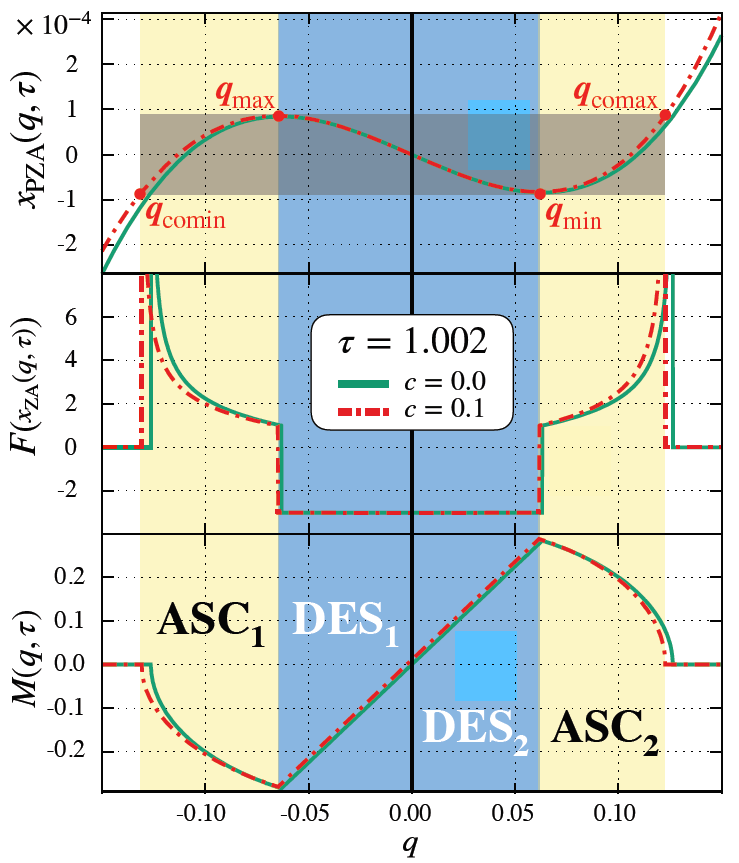
\includegraphics[scale=0.5, angle=0]{fig1.png}
		\caption{Immagine della mappa post-Zeldovich poco dopo il multistreaming, cioè a $\tau=1.002$}
		\label{fig:cmb}
	\end{figure}
\end{center}
